%% ****** Start of file apstemplate.tex ****** %
%%
%%
%%   This file is part of the APS files in the REVTeX 4 distribution.
%%   Version 4.1r of REVTeX, August 2010
%%
%%
%%   Copyright (c) 2001, 2009, 2010 The American Physical Society.
%%
%%   See the REVTeX 4 README file for restrictions and more information.
%%
%
% This is a template for producing manuscripts for use with REVTEX 4.0
% Copy this file to another name and then work on that file.
% That way, you always have this original template file to use.
%
% Group addresses by affiliation; use superscriptaddress for long
% author lists, or if there are many overlapping affiliations.
% For Phys. Rev. appearance, change preprint to twocolumn.
% Choose pra, prb, prc, prd, pre, prl, prstab, prstper, or rmp for journal
%  Add 'draft' option to mark overfull boxes with black boxes
%  Add 'showpacs' option to make PACS codes appear
%  Add 'showkeys' option to make keywords appear
\documentclass[aps,prl,twocolumn,groupedaddress]{revtex4-1}
%\documentclass[aps,prl,preprint,superscriptaddress]{revtex4-1}
%\documentclass[aps,prl,reprint,groupedaddress]{revtex4-1}

% You should use BibTeX and apsrev.bst for references
% Choosing a journal automatically selects the correct APS
% BibTeX style file (bst file), so only uncomment the line
% below if necessary.

\usepackage{graphicx}
\usepackage[caption=false]{subfig}
\usepackage{braket}
\usepackage{mathtools}
\graphicspath{{figures/}}
\DeclareMathOperator{\sinc}{sinc}

\begin{document}

% Use the \preprint command to place your local institutional report
% number in the upper righthand corner of the title page in preprint mode.
% Multiple \preprint commands are allowed.
% Use the 'preprintnumbers' class option to override journal defaults
% to display numbers if necessary
%\preprint{}

%Title of paper
\title{Force and Amplitude Sensing with Ions in a Penning Trap}

% repeat the \author .. \affiliation  etc. as needed
% \email, \thanks, \homepage, \altaffiliation all apply to the current
% author. Explanatory text should go in the []'s, actual e-mail
% address or url should go in the {}'s for \email and \homepage.
% Please use the appropriate macro foreach each type of information

% \affiliation command applies to all authors since the last
% \affiliation command. The \affiliation command should follow the
% other information
% \affiliation can be followed by \email, \homepage, \thanks as well.
\author{K. A. Gilmore}
\email[]{kevin.gilmore@colorado.edu}
%\homepage[]{Your web page}
%\thanks{}
%\altaffiliation{}
\affiliation{National Institute of Standards and Technology, JILA, and Department of Physics, University of Colorado, Boulder, Colorado, 80309, USA}

\author{J. G. Bohnet}
\author{J. J. Bollinger}
\affiliation{National Institute of Standards and Technology,, Boulder, Colorado 80305, USA}

%Collaboration name if desired (requires use of superscriptaddress
%option in \documentclass). \noaffiliation is required (may also be
%used with the \author command).
%\collaboration can be followed by \email, \homepage, \thanks as well.
%\collaboration{}
%\noaffiliation

\date{\today}

\begin{abstract}
This is where the abstract will go when I have one written.
\end{abstract}

% insert suggested PACS numbers in braces on next line
\pacs{}
% insert suggested keywords - APS authors don't need to do this
%\keywords{}

%\maketitle must follow title, authors, abstract, \pacs, and \keywords
\maketitle

% If in two-column mode, this environment will change to single-column
% format so that long equations can be displayed. Use
% sparingly.
%\begin{widetext}
% put long equation here
%\end{widetext}

% figures should be put into the text as floats.
% Use the graphics or graphicx packages (distributed with LaTeX2e)
% and the \includegraphics macro defined in those packages.
% See the LaTeX Graphics Companion by Michel Goosens, Sebastian Rahtz,
% and Frank Mittelbach for instance.
%
% Here is an example of the general form of a figure:
% Fill in the caption in the braces of the \caption{} command. Put the label
% that you will use with \ref{} command in the braces of the \label{} command.
% Use the figure* environment if the figure should span across the
% entire page. There is no need to do explicit centering.

% \begin{figure}
% \includegraphics{}%
% \caption{\label{}}
% \end{figure}

% Surround figure environment with turnpage environment for landscape
% figure
% \begin{turnpage}
% \begin{figure}
% \includegraphics{}%
% \caption{\label{}}
% \end{figure}
% \end{turnpage}

% tables should appear as floats within the text
%
% Here is an example of the general form of a table:
% Fill in the caption in the braces of the \caption{} command. Put the label
% that you will use with \ref{} command in the braces of the \label{} command.
% Insert the column specifiers (l, r, c, d, etc.) in the empty braces of the
% \begin{tabular}{} command.
% The ruledtabular enviroment adds doubled rules to table and sets a
% reasonable default table settings.
% Use the table* environment to get a full-width table in two-column
% Add \usepackage{longtable} and the longtable (or longtable*}
% environment for nicely formatted long tables. Or use the the [H]
% placement option to break a long table (with less control than 
% in longtable).
% \begin{table}%[H] add [H] placement to break table across pages
% \caption{\label{}}
% \begin{ruledtabular}
% \begin{tabular}{}
% Lines of table here ending with \\
% \end{tabular}
% \end{ruledtabular}
% \end{table}

% Surround table environment with turnpage environment for landscape
% table
% \begin{turnpage}
% \begin{table}
% \caption{\label{}}
% \begin{ruledtabular}
% \begin{tabular}{}
% \end{tabular}
% \end{ruledtabular}
% \end{table}
% \end{turnpage}


% body of paper here - Use proper section commands
% References should be done using the \cite, \ref, and \label commands
\section{Introduction}
% Put \label in argument of \section for cross-referencing
%\section{\label{}}

Introduction goes here.

\section{Experimental Setup}
In general, sensing an applied force requires a harmonic oscillator. Our harmonic oscillator  consists of the center-of-mass mode of $\prescript{9}{}{}$Be$^{+}$ ions confined to a single-plane Coulomb crystal in a Penning trap, described in Fig. 1 and (ref). The ions are cooled to the Doppler limit and the scattered fluorescence is used for imaging. The spin-1/2 system is the $\prescript{2}{}{S}_{1/2}$ ground state of the valence electron spin $\ket{\uparrow} (\ket{\downarrow}) \equiv \ket{m_{s}=+1/2} (\ket{m_{s}=-1/2}) $. In the magnetic field of the Penning trap, the ground state is split by 124 GHz. A resonant microwave source is used to perform global rotations of the spin ensemble. A pair of off-resonant laser beams generate a spin-dependent optical dipole force, coupling the spins to the ions's axial motion. The spins can be used as a sensitive readout of the axial motion.
\begin{figure}
  \subfloat[]{%
    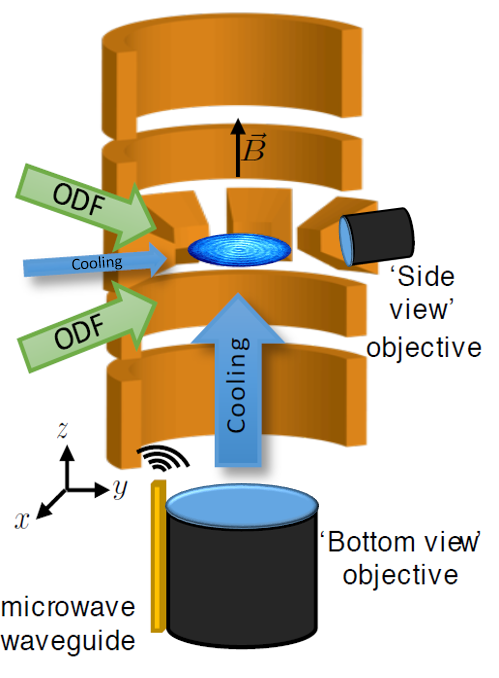
\includegraphics[width=.25\textwidth]{penning_trap}}\hfill
  \subfloat[]{%
    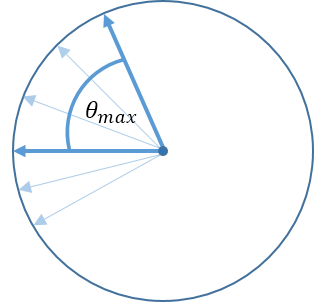
\includegraphics[width=.15\textwidth]{dumb_dephasing}}
  \caption{(a) Cross-section of the NIST Penning trap, characterized by an axial magnetic field $B = 4.45$ T and an axial trap frequency $\omega_z = 2\pi \times 1.57$ MHz. The blue disk represents the ion crystal. Cylindrical electrodes (orange) generate a harmonic confining potential along their axis. Radial confinement is provided by the Lorentz force from $\vec{E} \times \vec{B}$-induced rotation in the axial magnetic field. Time varying potentials applied to eight azimuthally segmented electrodes generate a rotating wall potential that controls the crystal rotation frequency. Doppler cooling beams are directed along $y$ and $z$. The beams responsible for the spin-dependent optical dipole force are at $10^{\circ} $ from the ion plane. Global, state-dependent fluoresence is collected on the side-view objective. (b) After rotating to the equator on the Bloch sphere, an incoherent axial perturbation causes precession. The maximum precessed angle is $\theta_{max}$. }\label{fig:1}
\end{figure}

By measuring the decrease in the composite Bloch vector length produced by the application of a homogenous spin-dependent force, detailed information about the motional state of the ions is revealed \citep{}. This spin dephasing is directly measured. The spin-dependent optical dipole force (ODF) is generated from the interference of a pair of detuned lasers, shown in Fig. 1a. The ODF couples the spin and motional degrees of freedom through the interaction 
\begin{equation}
H_{ODF} = U\sum_{i}\sin(\delta k \cdot z_i - \mu t + \phi)\sigma^{z}_i,
\end{equation}
where $z_i$ is the position operator for ion $i$ and $\mu/2\pi$ is the ODF laser beatnote frequency. This can be approximated as
\[H_{ODF} = U\sum_{i}\sin(\delta k \cdot z_i)\cos(\mu t + \phi)\sigma^{z}_i. \]
The precession due to an axial oscillation can be determined by considering a classical driven motion of constant amplitude and phase, $z_i \rightarrow z_i +z_0\cos(\omega t+\delta)$.
Then,
\[H_{ODF} = DWF \cdot U \cdot \delta k \cdot z_0\cos((\omega - \mu)t + \delta + \phi) \sum_{i} \frac{\sigma^{z}_{i}}{2} \]
where $DWF = \exp(-\delta k^2 \left< z^{2}_{i} \right> /2) $.
For $ \omega = \mu $,
\[\theta = \Delta\tau = DWF \cdot U \cdot \delta k \cdot z_0 \cdot \tau \cos(\delta - \phi) = \theta_{max}\cos(\delta - \phi)\]
where $\Delta$ is the energy difference between spin-up and spin-down for each ion.

We do our experiments phase incoherently (provide some motivation, ala Ozeri paper? or just explain that this is a limitation? probably both), but can extract the maximum precession angle, $\theta_{max}$. In a Ramsey sequence where the Bloch vector with no precession is rotated down to the dark state, the component along $-\hat{z}$ has length $\cos(\theta)$. Thus the probability for measuring spin-up is $P_{\uparrow} = \frac{1}{2}[1-e^{-\Gamma \tau} \cos(\theta)]$, where $\tau$ is the total ODF interaction time and $\Gamma = \frac{1}{2}(\Gamma_{el} + \Gamma_{ram})$ is the spontaneous decay rate where $\Gamma_{el}$ ($\Gamma_{ram}$) is the elastic (Raman) scattering decoherence rate (Uys PRL ref). To model the phase incoherent experiment, one must average over this length, $ \left< \cos(\theta) \right> $. It can be shown that $ \left< \cos(\theta) \right> = J_0(\theta_{max}) $, where $J_0$ is the zeroth order Bessel function of the first kind. Thus,
\begin{equation}
\left< P_{\uparrow} \right> = \frac{1}{2} [1-e^{-\Gamma \tau}J_0(\theta_{max}).
\end{equation}
To create an axial oscillation, we apply an AC voltage (RF potential?) to the endcap of the Penning trap. This can be done either on-resonance or off-resonance with the center of mass mode of the ion crystal at $2\pi \times 1.57$ MHz. To calibrate the displacement of the ions as a result of this applied drive, we apply a static voltage to the endcap and measure the deflection of the ion crystal. From this calibration, we find 1 mV results in 1 nm of displacement.

\section{Off-resonance amplitude sensing}

\begin{figure}
\centering
  \subfloat[]{%
    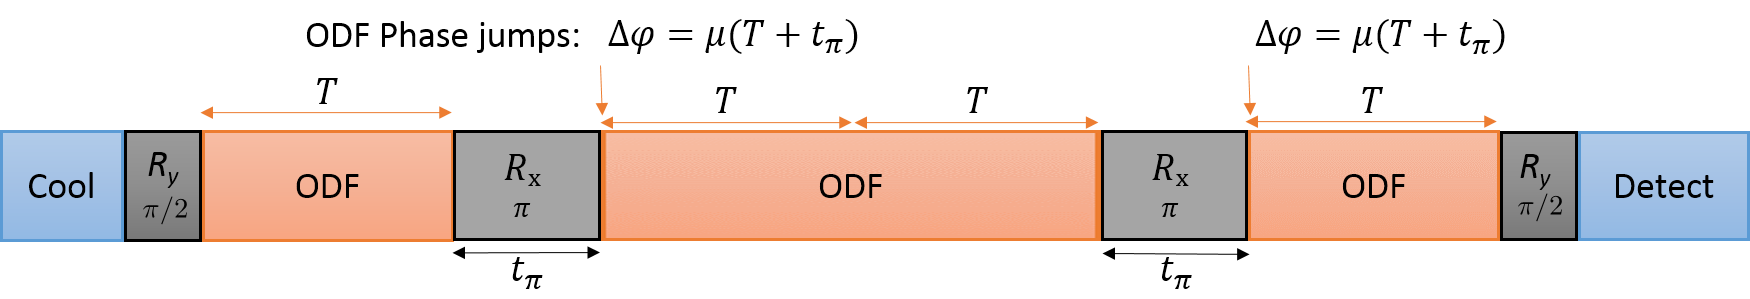
\includegraphics[width=.5\textwidth]{cpmg}}\\
  \subfloat[]{%
    
\includegraphics[width=.5\textwidth]{8pi_cpmg}}\\
  \subfloat[]{%
    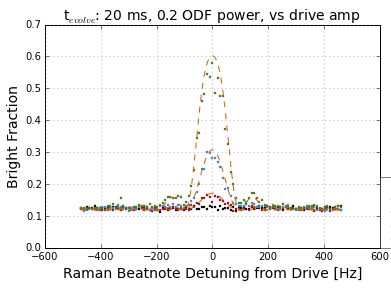
\includegraphics[width=.24\textwidth]{lineshape_vs_drive}}\hfill
  \subfloat[]{%
    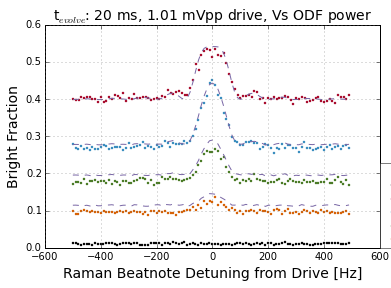
\includegraphics[width=.24\textwidth]{lineshape_vs_odf}}\\
  \subfloat[]{%
    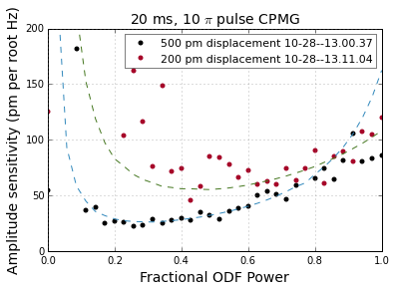
\includegraphics[width=.25\textwidth]{amp_sense_both}}
  \caption{(a) CPMG sequence with 2 $\pi$ pulses. Orange blocks represent ODF pulses, grey microwave rotations, and blue cooling and detecting. In this experiment, the classical drive is left on throughout. After each $\pi$ pulse, the ODF phase is jumped in order to sum the phases accumulated in each ODF arm. (b) CPMG sequence with 8 $\pi$ pulses. Cooling and detection remain the same, and the phase is jumped by the same amount after each pi pulse. Chaining the ODF pulses in this fashion allows us to go to much longer total interaction times (20 ms) and detect much smaller induced displacements.   (c) Lineshape of the classical drive for several drive amplitudes. Black points are background, with drive turned off. Dashed lines are theory curves with no free parameters.  (d) Lineshape for fixed classical drive and various ODF powers. As the ODF power is increased, the background rises and the optimal signal-to-noise is found. (e) Amplitude sensitivity as a function of ODF power. There is an optimal signal-to-noise that occurs before the background begins to dominate. We calculate a minimum sensitivity of ~25 pm per root Hz.}\label{fig:2}
\end{figure}

By applying a ~400kHz drive to the endcap electrode, we can study the response of the ion harmonic oscillator to an off resonant force. A spin echo sequence is used to decouple from magnetic field fluctuations over the course of the experimental sequence. To extend the sequence out to long time in order to detect more sensitively, a CPMG style sequence is used. Our experimental sequence makes use of the quantum lock-in technique wherein the phase accumulated in each arm of the sequence is added coherently. Figure () shows a CPMG sequence with 2 $\pi$ pulses and phase jumps appropriate for adding the phases. Adding in 6 additional $\pi$ pulses and ODF pulses allows us to push the sequence time out to 20 ms and maintain a background fully characterized by decoherence due to spontaneous emission. For this experiment, the drive is left on continuously.

To model the lineshape of the signal, it is necessary to account for the accumulated phase due to the spin-dependent ODF potential without making the simplification that $ \omega = \mu $. This results in a characteristic response function for each sequence. For the 8 $\pi$ pulse CPMG sequnce
%\begin{widetext}
%\begin{equation}
%\theta_{tot} = \theta_{max} \left[ \frac{2 \sin(\frac{1}{2}[(\omega-\mu)T])}{\omega-\mu} \right] 
%\left[ \sin(\frac{\omega}{2}(T+t_{\pi})) \right] \left[ \sin(\frac{1}{2}[\omega (T+t_{\pi}) + (\omega - \mu)T)]) \right] \left[ \cos(\omega(T+t_{\pi})+(\omega - \mu)T) \right] \left[ \cos(2(\omega(T+t_{\pi})+(\omega - \mu)T)) \right] 
%\end{equation}
%\end{widetext}

\begin{widetext}
\begin{equation}
\theta_{tot} = \theta_{max} \left[ \sinc \left( \frac{T}{2} \left( \omega-\mu \right) \right) \right] 
\left[ \cos \left( \frac{T}{2} \left( \omega - \mu \right) \right) \right] \left[ \cos(T(\omega - \mu)) \right] \left[ \cos(2T(\omega - \mu)) \right] 
\end{equation}
\end{widetext}
Fig 2c shows the emergence of the signal out of the background as the drive amplitude is increased. Fig 2d shows the evolution of the signal relative to the background as the power of the ODF beams is increased. In both cases the theory has no free parameters.

With the drive frequency chosen to correspond to the peak signal, scanning the power of the ODF laser varies the strength of the measurement. For particular drive amplitudes, by comparing the curve to the background, the signal and the signal-to-noise can be extracted. From this, the sensitivity of the sequence is found. To calculate the signal-to-noise ratio, a value for $\theta_{max}$ needs to be extracted. Taking the difference between $\left< P_{\uparrow} \right>$ with the classical drive applied and $\left< P_{\uparrow} \right>_{bckgnd}$ with no drive and solving for $J_0(\theta_{max})$ yields
\[J_0(\theta_{max}) = 1 - 2e^{\Gamma \tau} \left[ \left< P_{\uparrow} \right> - \left< P_{\uparrow} \right>_{bckgnd} \right] \]
The signal-to-noise for a single experiment is given by $S/N =\theta_{max}/\delta \theta_{max}$, where $\delta \theta_{max} \equiv \delta J_0(\theta_{max})/ \left( \frac{dJ_0(\theta_{max})}{d\theta_{max}} \right)$. To get the per-root-Hz sensitivity, the amplitude of the displacement - gotten from the calibration with a known applied drive voltage - and the measurement bandwidth is used. $sense = z_d\sqrt{\tau}/SNR$. Fig 2e shows the amplitude sensitivity as a function of measurement strength.

We have measured amplitudes as small as 200 pm, a fraction of the extent of the ground state wavefunction of the ion crystal (10 nm). The amplitude sensitivity is $\sim$30 pm/ $ \sqrt{Hz}$.

\section{On-resonance force sensing}

An RF drive at $2\pi \times 1.57$ MHz produces a resonant excitation of the center-of-mass mode. On resonance, the experiment is much more sensitive to applied forces. The experimental sequence consists of two ODF arms with the classical drive pulsed on between and a $\pi$ microwave pulse halfway through. The $\pi$ pulse serves to reduce dephasing due to magnetic field fluctuations. The second ODF pulse is the readout for the spin dephasing caused by the applied drive. The first ODF pulse provides cancellation of coherent thermal fluctuations that result in spin dephasing, as well. Because this experiment is done on-resonantly it is more sensitive to these effects, as well as fluctuations in the COM mode frequency. We find that this sequence does not perfectly cancel thermal fluctuations and we end up with a background far above that predicted from spontaneous emission alone. As a result, the duration of the sequence cannot be extended in the same way as the off-resonant sequence. Thus, we are limited to sensing amplitudes on the order of the size of the ground state wavefuntion - 10 nm. However, the smallest observed per-ion force is $\sim$0.75 yN \citep{Biercuk2010a}. 

By shortening the drive time to its minimum - the microwave $\pi$ time - the smallest possible displacement may be detected. Then, by lowering the drive amplitude and increasing the drive time - allowing the displacement amplitude to ring up - the smallest measurable force may be detected. Fig 3b shows the increase of the signal as a function of the drive time. Fig 3c shows as a function of ODF power the background with no classical drive applied, a small drive applied, and the relevant theory curves. We fit the background to a Gaussian and use this in the theory calculation for the signal \cite{Ivanov2016c}.
\begin{figure}
\centering
  \subfloat[]{%
    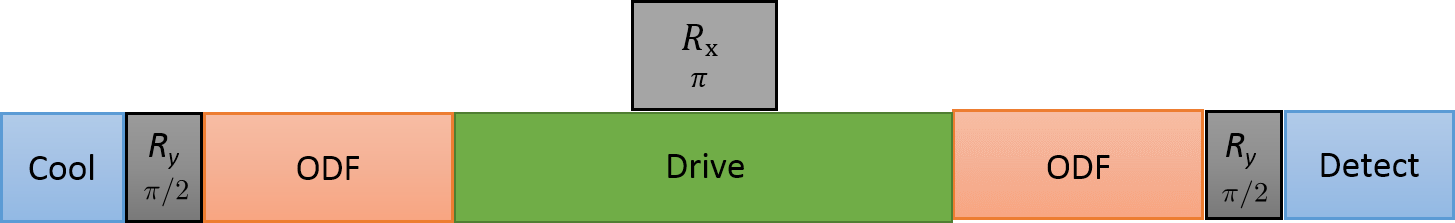
\includegraphics[width=.5\textwidth]{onres_seq}}\\
  \subfloat[]{%
    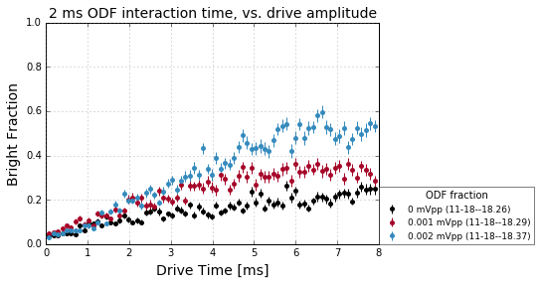
\includegraphics[width=.24\textwidth]{on_res_drive_t}}\hfill
  \subfloat[]{%
    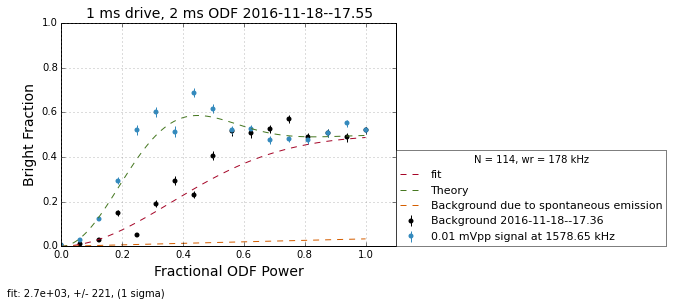
\includegraphics[width=.24\textwidth]{on_res_odf_scan}}\hfill
  \subfloat[]{%
    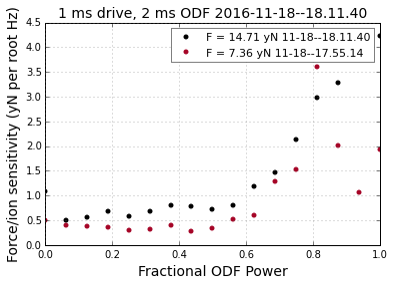
\includegraphics[width=.25\textwidth]{force_sens}}\\    
  \caption{(a) Experimental sequence for on-resonance sensing. The classical drive is not on while the ODF beams are. A pi pulse in the middle of the sequence provides a spin-echo, eliminating dephasing due to magnetic field fluctuations. The second ODF pulse is the readout for the amplitude of oscillation caused by the drive. The first ODF pulse completes the symmetry and cancels coherent thermal fluctuations across the sequence. (b) Increasing the length of the drive allows the oscillation amplitude to ring up. By going to longer drive times, sub-yN forces can be resolved. Black points are the background, with no drive on. (c) Background and signal as a function of ODF power. Red curve is a fit to a Gaussian. Green curve is theory with the background fit taken into account. (d) Force sensitivity vs ODF power.}\label{fig:3}
\end{figure}

\section{Conclusion}
And to conclude: the conclusion.

\subsection{}
\subsubsection{}


% Specify following sections are appendices. Use \appendix* if there
% only one appendix.
%\appendix
%\section{}

% If you have acknowledgments, this puts in the proper section head.
%\begin{acknowledgments}
% put your acknowledgments here.
%\end{acknowledgments}

% Create the reference section using BibTeX:
\bibliographystyle{apsrev4-1}
%\bibliographystyle{apalike}
\bibliography{force_sensing}

\nocite{}
\end{document}